\chapter{Restricted team selection}
\label{chap:bounded}
Several Leagues (and some Research tasks) place a ceiling on the CP of
 participating Pokémon.
We have established that CP is a poor proxy for PvP performance, and thus
 expect that we might find strong candidates based on where CP fails.
If CP does not accurately represent a given Pokémon's chance to win, we ought
 be able to exploit this by assembling teams using undervalued Pokémon\footnote{Michael Lewis might call it ``Moneymon''.}.
We first take the sorted list of Pokémon developed in \autoref{chap:unbounded},
 and remove all entries not in the optimal sets generated below.
We then select a team using the strategies of that chapter. Since
 that list was sorted according to a general strength function, it
 ought apply in this reduced context.
\textbf{This chapter has no relevance for Nx1 battles, nor the Master
  League, none of which employ CP bounds.}

\section{Optimal IVs and Levels under a CP bound}
We require a fitness function that takes as input a Pokémon's form, level, and IV,
  and emits a comparable output.
Common functions include CP itself, the arithmetic mean ($\frac{Eff_A +Eff_D + MHP}{3}$),
  and the geometric mean ($\sqrt[3]{Eff_A \times Eff_D \times MHP}$)\footnote{I personally believe the geometric mean to best match Pokémon GO's
  mechanics, but there is no true ``best'' fitness function---optimal IVs are
  dependent upon both the base stats and the opponent.}.
For a given CP bound, fitness function, and form, there is some optimal set of Pokémon levels
 and individual vectors.
Higher IV components might require a lower level than lower components to
 come in under the same ceiling.
What can be said is that IVs add less value to a high base stat than a low
 base stat, and that higher levels provide diminishing returns.
For a base stat of 100, a corresponding IV component of 15 represents a
 15\% improvement to $Eff_A$.
For a base stat of 300, the same IV represents only a 5\% improvement.
A Level 10 Pokémon advancing to level 10.5 enjoys a 2.47\% improvement to
 $Eff_A$ (and also $Eff_D$ and $Eff_S$), paying a price of 5\% increase
 in CP.
Advancing from 30 to 30.5 represents only a 0.42\% improvement (and a
 0.83\% increase in CP).

The maximum level for which a 15--15--15 IV comes in under the bound is the
 minimum possible optimal level, since any lesser level would be strictly less
 powerful.
The maximum level for which a 0--0--0 IV comes in under the bound is the
 maximum possible optimal level, as it is not possible to gain another level
 while remaining within the bound.
Any IV with all three components less than or equal to another IV, but bounded
 by the same level, is strictly inferior to the second IV, and can be discarded.
Compute $Eff_A$, $Eff_D$, and $MHP$ using the IVs and corresponding levels.
Any resulting set with all three components less than or equal to some other set's
 is strictly inferior to the second, and can be discarded.
This captures $MHP$'s floor function.
What remains is an optimal frontier of at least one solution (usually
 many solutions), where arguments can be made for each depending on how one
 values attack, defense, and stamina, especially in the context of different
 opponents.

Before taking Power and Type into the question, let's examine the optimal
 solutions for a genus using the 1500 and 2500 CP bounds, using the
 geometric mean of $Eff_A$, $Eff_D$, and $MHP$ as our global fit function.
Timburr (134 ATK, 87 DEF, and 181 STA) evolves into
  Gurdurr (180 ATK, 134 DEF, and 198 STA), which evolves into
  Conkeldurr (243 ATK, 158 DEF, 233 STA).
Their base products are 2,110,098 (Timburr), 4,775,760 (Gurdurr),
  and 8,945,802 (Conkeldurr).
The geometric means are 128.263, 168.402, and 207.590.
Poor Timburr isn't really suited for the common PvP Leagues,
  and does best with a 15--15--15 at Level 50 (CP 1487).
Gurdurr can hold its own under a 1500 CP ceiling, and its
  optimal IVs are 1--15--15 at Level 26 (CP 1496).
It falls short of the Ultra League's 2500, though, where
  15--15--15 and 15--15--14 are functionally equivalent
  at Level 50 (both result in MHP of 178) despite
  respective CPs of 2452 and 2447.
It is impossible to distinguish between a Level 16.5 Conkeldurr at
  3--15--15 or 3--15--14 (134 MHP either way), though
  the CPs are 1500 and 1497.
In the Ultra League, Conkeldurr wants Level 28 0--15--12 with
  a CP of 2499.
Take two things away from this:
\begin{itemize}
\item The optimal IVs, and even the number of equivalent optimal IVs, can change across evolution.
  This is largely independent of any global fitness function.
\item Hitting the ceiling does not guarantee optimal IVs for most fitness functions.
  More generally, under most fitness functions, higher CP does not necessarily imply superior IVs.
    Gurdurr has numerous solutions yielding 1500 CP (3/2/0@28, for instance, with geometric
    mean 120.015), but 1/15/15@26 beats it at 1496 (121.968).
\end{itemize}
There are many fitness functions. In the Gurdurr example given previously, 3--2--0 loses
    to 1--15--15 at geometric mean, but has an $Eff_A$ of 129.36, comfortably above the latter's 123.29.
 Does this compensate for six fewer hit points (145 vs 139) and lower $Eff_D$ (101.49 vs 96.136)?
 Let's pit them against one another, using Low Kick (Power of 4, neutral type effectiveness, STAB bonus).
 Our Level 28 competitor strikes for six damage with each attack:
    \[ \left\lfloor \frac{129.36 \times 4 \times 1.2}{101.49} \right\rfloor = \lfloor 6.118 \rfloor = 6 \]
 The supposedly optimal Gurdurr strikes for six as well:
    \[ \left\lfloor \frac{123.29 \times 4 \times 1.2}{96.136} \right\rfloor = \lfloor 6.156 \rfloor = 6 \]
 At 145 HP, Gurdurr goes down on the 25th attack.
 Its opponent's 139 HP absorbs 23 attacks before falling to the 24th, but this could
    have easily gone the other way.
 If the attack's Power were 10, both hit for nine damage, and both fall after nine attacks.

\section{Optimal League forms}
Pokémon GO offers two CP-bounded PvP leagues, the Great League (CP 1500) and
   the Ultra League (CP 2500).
\textbf{FIXME: update this for new lists}
\autoref{table:cp1500} lists species' optimal level and IVs for the Great League
  as evaluated using the geometric mean of $Eff_A$, $Eff_D$, and $MHP$.
Species which can't manage a geometric mean of 95 have been left out.
\autoref{table:cp2500} does the same for the Ultra League, eliding those species which
  can't hit a $\sqrt[3]{BP}$ of 130.
A few observations from the CP1500 table:
In general, there is no correlation between $\sqrt[3]{BP}$ and level,
  save that everything at the bottom of the list is maxed (15/15/15@50),
  since many species cannot reach 1500 CP at all.
The geometric mean ($\sqrt[3]{BP}$) ranges from 51.39 (max Shedinja)
  to 147.18 (15/15/15@49.5 Chansey).
There is a strong bimodal preference for IVs: 15/15/15 for level 49.5
  and 50, and otherwise $n$/15/15 where $n < 2$, and $n$ usually equals 0.
This verifies (not that we had any doubt) that attack is highly overvalued in the CP calculation relative to $\sqrt[3]{BP}$.
Other IVs usually correspond to low level, powerful species, where a level
  raises CP by a large amount, leaving more room for beneficial IVs.
$Eff_A$ ranges from 63.02 (Chansey) to tremendous outlier 254.05 (Deoxys Attack).
In general, the top positions have relatively low $Eff_A$, rising in an
  orderly fashion to about 145 as we go down the list.
At this point, they become more disordered, until falling at the back
  of the list.
$MHP$ and $Eff_D$ are much less predictable.
\begin{figure}[h]
\begin{minipage}{0.5\textwidth}\begin{center}
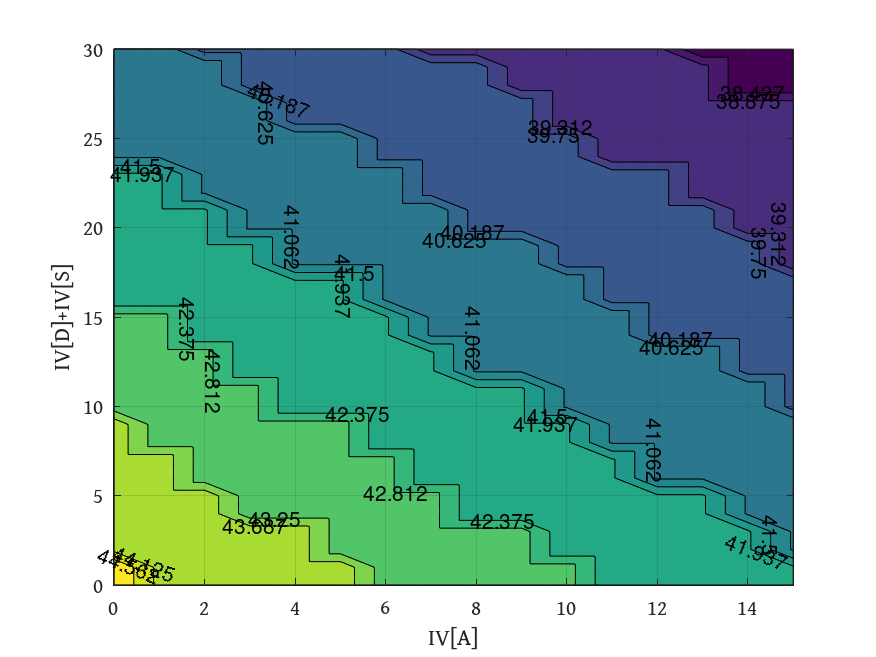
\includegraphics[width=\textwidth,keepaspectratio]{octave/greninjalevels.png}
\end{center}\end{minipage}%
\begin{minipage}{0.5\textwidth}\begin{center}
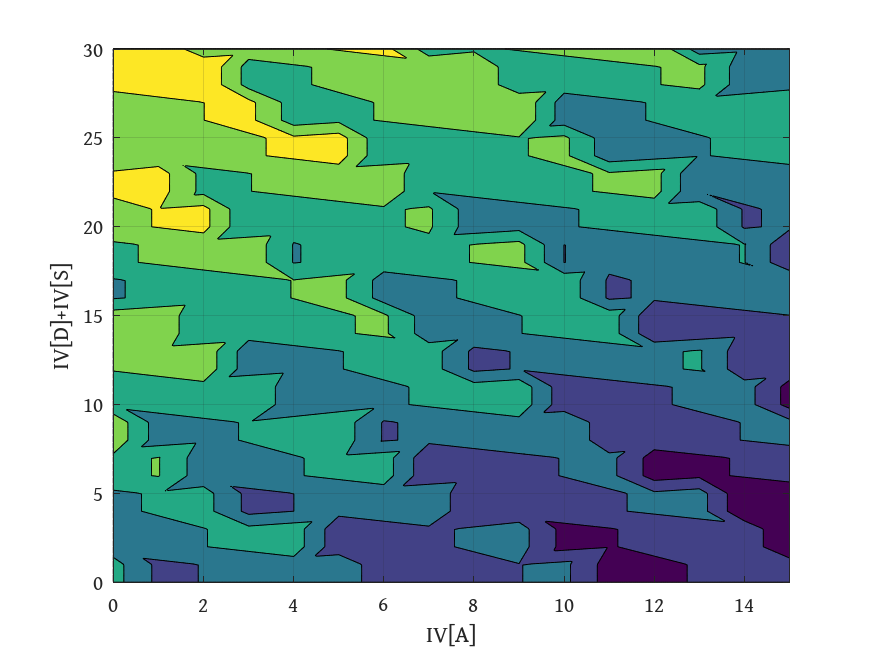
\includegraphics[width=\textwidth,keepaspectratio]{octave/greninjagmeans.png}
\end{center}\end{minipage}%
\caption[Contours of optimal Greninja levels]{Contours of optimal Greninja levels and resulting geometric means
  (X axis is $IV_A$, Y axis is $IV_D + IV_S$).}
\label{fig:contours}
\end{figure}
What's more important, IVs or level?
Given the vast number of 0/15/15 IVs among the optimal sets, it
  would seem to be $IV_D$ and $IV_S$ (and that it is equally
  important to minimize $IV_A$).
This is true for levels below 30 or so, but more powerful Pokémon
  have optimal configurations below that.
Among these, we see much more diversity of IVs.
The IVs are being pushed lower to allow for higher levels.
This reflects the diminishing returns on CPM as level increases.
The real answer is: equal importance until level 30 or so, and IVs beyond that,
  though the Attack component is always less important than level
  (as evidenced by the large number of x/15/15@50 configurations).

What's always more important is typing and attack selection.
I'm a fan of bringing in powerful Pokémon at low levels; their stats are
  comparable to less powerful Pokémon at higher levels, but they
  generally have more powerful moves.
One has to be careful choosing, though; most end up woefully underpowered
  with respect to MHP vs potential MHP (\autoref{fig:maxmhpvsoptmhp}).
\begin{figure}
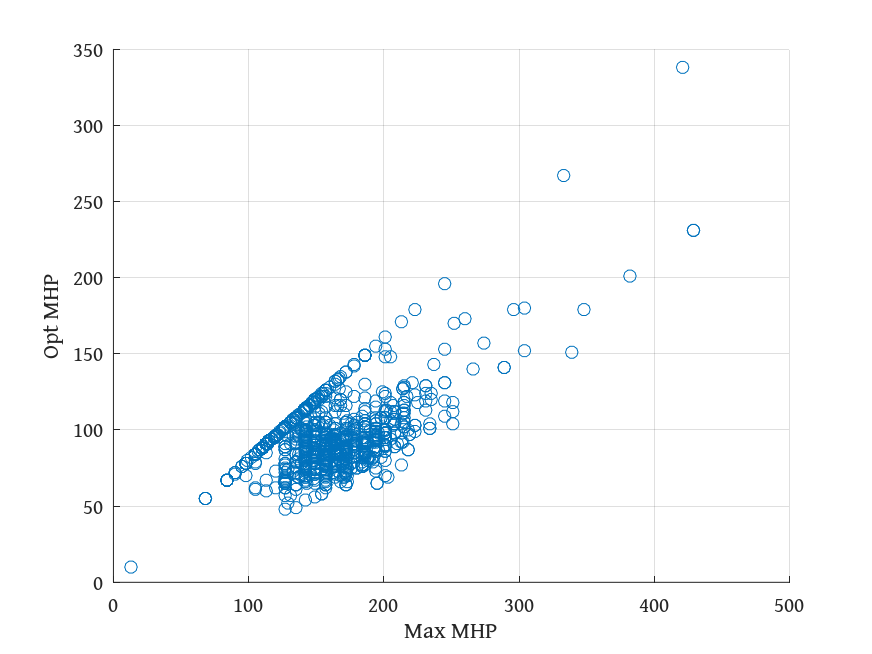
\includegraphics[width=\textwidth]{octave/maxmhpvsoptmhp.png}
\caption{$\frac{BS}{3}$-optimal MHP vs maximum possible MHP.}
\label{fig:maxmhpvsoptmhp}
\end{figure}

\section{Anticipating opponents}
Similarly to an unbounded contest, we can assume that a rational opponent is selecting
  according to the same rules as we are (or better), but a more powerful result is
  strong against all possible opponents.
\textbf{FIXME}

\section{Breakpoints}
\label{sec:breakpoints}
Should you have (or believe you have) a good idea of what you'll be going up against,
 breakpoint analysis is a powerful tool.
Essentially, we want to model the relationship between two Pokémons' $Eff_D$
 and $Eff_A$ \textbf{FIXME exact stat from earlier equations}.
Alternately, we want to model damage inflicted against MHP.
Using this information, we can perhaps choose more optimal IVs and levels for a given CP bound.
Of course, this is only as useful as the accuracy of our information, and how narrow a set of opponents it specifies.

In \autoref{table:bpoints1} and \autoref{table:bpoints2}, we see level 50 Clodsire
  employing two charged attacks against level 50 Sawk.
Columns correspond to different $IV_A$ for Clodsire, and rows to different $IV_D$ for Sawk.
The spread of damage is greater for Earthquake than Megahorn (16 versus 9), a ratio
  of 1.\textoverline{7}, significantly more than the ratio of Earthquake (with STAB)
  to Megahorn (1.2).
I haven't included a table for fast attack, as it deals damage of 2 for all combinations of IVs.

\textbf{FIXME}
\input{out/breakpoints}

\section{Type restrictions}
\label{sec:typeleagues}
A common variation on the usual Leagues is a type restriction.
The summer of 2025 features the ``Fossil Cup'', wherein all competing
  Pokémon (in addition to coming in under the CP1500 bound)
  must include Rock, Steel, or Water in their typing.
The cover sets of \autoref{sec:coversets} make their return with a vengeance!

We can cover these three types with just two attack types: Fighting and Grass, or Grass and Ground.
Indeed, all three of these types are strong against two of the target types.
Two sets of six attack types fully cover these typings.
We could stripe these across the two charged attacks of three Pokémon,
  leaving our fast attacks free, or stripe them across the six total
  attacks of two Pokémon, leaving the third free.
Or we could double up.
I'll develop this more fully in \autoref{chap:example}.
